%!TeX program=pdflatex
%!TeX encoding=utf8
%!TeX spellcheck = en_US
%!TeX root = ../../messageVortex.tex

\partepigraph{No matter how hard you work, someone else is working harder.}{Elon Musk, entrepreneur}
\part{Implementation\label{sec:implementation}}
\fxwarning{Insert implementation details and real world problems}

\chapter{Security Related decisions}
As we decided earlier to stick with an agile set of algorithms, a suitable choice had to be made for the reference implementation. Multiple interests were taken into account. The algorithms should be efficient, researched (if possible) and a reference implementation in Java should be available. The last criteria was easy to fulfill, as most of the algorithms had already a reasonable implementation in java.

When looking into research, we discovered that the choice is very hard to be made. Some algorithms (e.g., modes or paddings) had even properties which allowed to leak information (e.g., due to authentication). This is why our choice took more efforts than originally planed.

\section{Chunking and Padding of Message Blobs}

	
\section{Algorithm Choice}
\subsection{Choice of Cryptographic Algorithms, Modes and Paddings}
\subsection{Choice of PRNGs}
\subsection{Choice of Steganographic Algorithms}
\section{Chunking of Plain Embedded Messages}\label{sec:chunkingPlain}

\section{Side Channel Leaking}
\subsection{Software Updates and Related Data Streams}
\subsection{Bugging in transported messages}


\chapter{Usability Related Implementation Details}
\section{Adressing and address representations}
\section{Linking to Common User Agents}

\chapter{Efficiency Related Implementation Details}
\section{Node Storage Management}
\subsection{Life-cycle of Ephemeral Identities and Workspaces}
\subsection{Life-cycle of Requests}
\subsection{Life-cycle of Operations}
\section{ASN.1 encoding scheme}
Originally, we implemented the protocol as XML encoded messages. This encoding had, however, several flaws. First the huge ammount of encrypted data within the document made the messages bulky and at the same time loose one of its main strengths: readability for humans. The encoding required for binary data caused messages to increase ion size due to their onionized structure. 

Furthermore, the complex XML features \fxwarning{incomplete section}

\section{Processing of messages}

\subsection{Processing of Incoming Messages}\label{sec:processingIncommingMessages}
A Block is picked up in the blending layer and then handled in the routing layer. First, we try to authenticate the message. If we can authenticate the message, we process it and add the contained instructions to a processing workspace. Unauthenticated messages may be discarded at any point.

The processing of a sending block is triggered by a routing block in the workspace, as shown in figure~\ref{fig:msgSendProcessing}. The assembly instructions are processed to collect the payload blocks. Then the encryption is applied to the message and passed on to the blending layer for processing.

\begin{figure*}[hbt]
	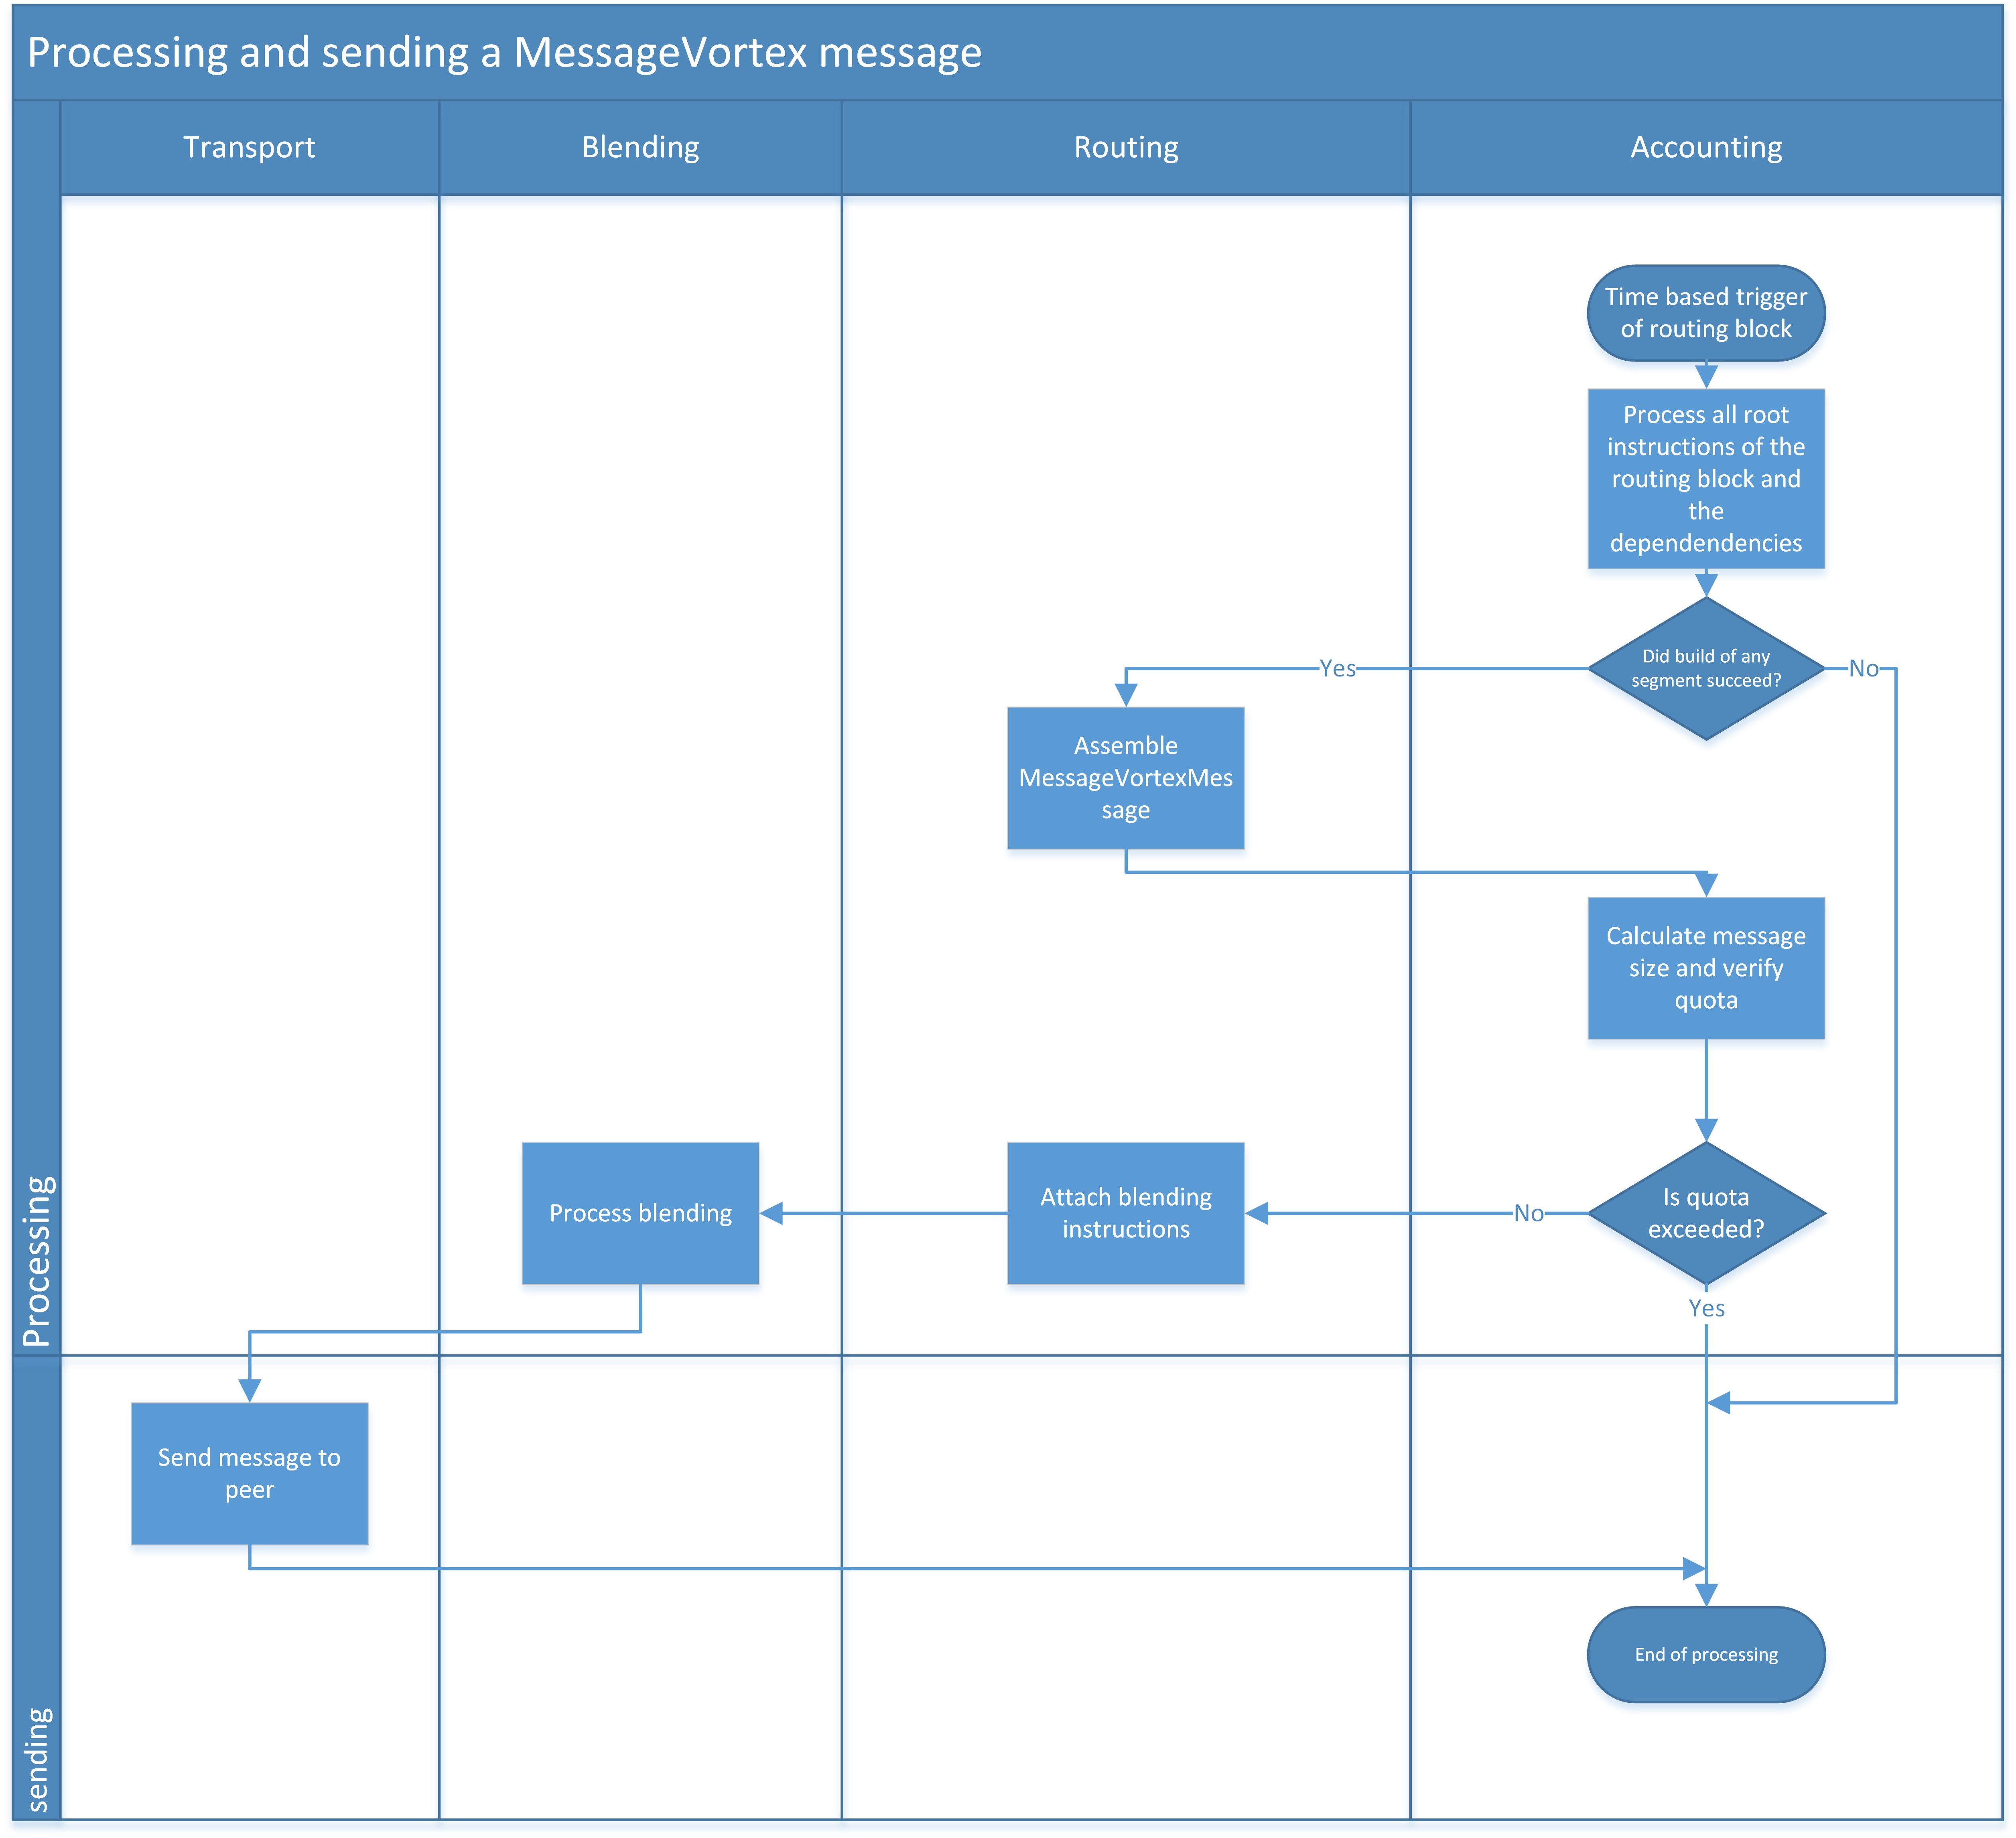
\includegraphics[width=0.90\textwidth]{inc/flowchart_message_sending}
	\caption{flow diagram showing processing of outgoing messages}
	\label{fig:msgSendProcessing}
\end{figure*}

\fxwarning{complete section}

\subsection{Processing of Outgoing Messages}\label{sec:processingOutgoingMessages}
\fxwarning{complete section}

\subsection{Implementation of Operations}\label{sec:implOperations}
\fxwarning{Mention mapping operation}

\fxwarning{Mention floating point issues when splitting}

\fxwarning{complete section}

\section{Request handling}
\fxwarning{complete section}

\subsection{Requesting a new Ephemeral Identity}\label{sec:newEID}
\fxwarning{complete section}

\subsection{Replacing an Existing Node Identity}
\fxwarning{complete section}

\subsection{Replacing an Existing Reply Block}\label{sec:replaceMURB}
\fxwarning{complete section}

\subsection{Updating the Software}
\fxwarning{complete section}
